% mlxforge --- Technical White Paper
% Build: latexmk -pdf mlxforge-whitepaper.tex   (or: make)
\documentclass[11pt,a4paper]{report}

% --- math ---
\usepackage{amsmath}
\usepackage{amssymb}
\usepackage{mathtools}

% --- layout / typography ---
\usepackage[a4paper,margin=1in]{geometry}
\usepackage{microtype}
\usepackage{enumitem}
\usepackage{fancyhdr}
\usepackage{booktabs}
\usepackage{array}
\usepackage{longtable}
\usepackage{graphicx}
\usepackage{xcolor}

% --- code listings ---
\usepackage{listings}

% --- diagrams ---
\usepackage{tikz}
\usetikzlibrary{positioning,arrows.meta,fit,backgrounds,calc,shapes.geometric}

% --- bibliography ---
\usepackage[numbers,sort&compress]{natbib}

% --- hyperref last ---
\usepackage[colorlinks=true,linkcolor=black!70!blue,citecolor=black!60!green,urlcolor=black!60!blue]{hyperref}

% ---------------------------------------------------------------------------
% styling
% ---------------------------------------------------------------------------
\definecolor{codebg}{rgb}{0.97,0.97,0.97}
\definecolor{codekw}{rgb}{0.10,0.10,0.55}
\definecolor{codecm}{rgb}{0.30,0.45,0.30}
\definecolor{codestr}{rgb}{0.55,0.20,0.10}

\lstdefinestyle{mlxforge}{
  backgroundcolor=\color{codebg},
  basicstyle=\ttfamily\footnotesize,
  keywordstyle=\color{codekw}\bfseries,
  commentstyle=\color{codecm}\itshape,
  stringstyle=\color{codestr},
  numberstyle=\tiny\color{black!50},
  numbers=left,
  numbersep=7pt,
  frame=single,
  rulecolor=\color{black!20},
  breaklines=true,
  showstringspaces=false,
  tabsize=2,
  captionpos=b,
  columns=fullflexible,
  keepspaces=true,
}
\lstset{style=mlxforge}
\lstdefinelanguage{none}{keywords={},sensitive=true,morecomment=[l]{\#}}

% absorb unbreakable monospace tokens (long file paths) without ragged right
\emergencystretch=3em

\pagestyle{fancy}
\fancyhf{}
\fancyhead[L]{\small\itshape mlxforge}
\fancyhead[R]{\small\thepage}
\renewcommand{\headrulewidth}{0.3pt}

% notation shortcuts
\newcommand{\R}{\mathbb{R}}
\newcommand{\code}[1]{\texttt{#1}}
\newcommand{\softmax}{\operatorname{softmax}}
\newcommand{\silu}{\operatorname{SiLU}}
\newcommand{\rmsnorm}{\operatorname{RMSNorm}}
\newcommand{\rope}{\operatorname{RoPE}}
\newcommand{\elemmul}{\odot}

% ===========================================================================
\begin{document}

\begin{titlepage}
  \centering
  \vspace*{2cm}
  {\Huge\bfseries mlxforge\par}
  \vspace{0.6cm}
  {\Large A Batched, Embeddable LLM Inference Engine on Apple MLX\par}
  \vspace{0.4cm}
  {\large Architecture, Numerics, and Software Design\par}
  \vspace{2cm}
  {\large Technical White Paper\par}
  \vspace{0.3cm}
  {\normalsize Engine version: continuous-batching core, C ABI v7\par}
  \vfill
  {\small This document consolidates the design of the \code{mlxforge} engine: the
  product thesis, the threading and continuous-batching model, the mathematics of
  the transformer forward pass and its model-family variants, the Qwen3-VL vision
  pipeline, the stable C ABI and cross-language bindings, and the
  golden-reference testing methodology.\par}
  \vspace{1cm}
  {\small\today\par}
\end{titlepage}

% ---------------------------------------------------------------------------
\begin{abstract}
\noindent
\code{mlxforge} is a from-scratch C++17 inference engine built directly on the
Apple MLX C++ array library (not \code{mlx-lm}), targeting Apple Silicon through
the Metal backend. It serves LLaMA-family decoder models (Llama-3.2, Qwen3
dense/MoE, Qwen3.5 hybrid) and the Qwen3-VL vision-language model, with
\emph{continuous batching}: many concurrent requests share one resident model and
one GPU worker, dynamically admitted and evicted from an active batch. The KV
cache can be stored quantized (8- or 4-bit, mirroring \code{mlx-lm}'s
\code{QuantizedKVCache}), and an opt-in prefix cache pools immutable KV blocks
keyed by a salted chain hash of the token prefix --- with an SSD spill tier that
survives engine restarts --- so requests sharing a system prompt or a
conversation history skip recomputing the shared span.

The engine occupies a specific gap in the Apple MLX ecosystem. Single-stream
libraries (\code{node-mlx}, Apple's \code{MLXLLM}) cannot batch; batched servers
(\code{vllm-mlx}, \code{omlx}) are Python processes reachable only over HTTP.
\code{mlxforge} is simultaneously \emph{in-process}, \emph{MLX-native}, and
\emph{batched}, exposed through a stable C ABI so it can be embedded from Node,
Swift, and Rust as a shared library. The product is that library, not the bundled
HTTP server or CLI.

The defining engineering constraint is that the failure mode of an inference
engine is \emph{silent numerical garbage, not a crash}. So every numerically
sensitive stage (embedding, RoPE, attention masking, the per-layer forward,
sampling, and the full vision pipeline) is gated against \code{.npy} golden
fixtures dumped from the \code{mlx-lm}/\code{mlx-vlm} reference running the same
weights, and greedy decoding has to match token-for-token. This paper documents
the architecture and the mathematics in enough detail to reproduce or audit the
implementation.
\end{abstract}

\tableofcontents

% ===========================================================================
\chapter{Introduction and Thesis}
\label{ch:intro}

\section{What mlxforge is}
\code{mlxforge} is an embeddable local-inference engine written in C++17 on top of
the Apple MLX core array library. It runs autoregressive decoder language models
on Apple Silicon GPUs via Metal, and it does so with continuous batching: a single
resident copy of the model weights and a single GPU worker thread serve many
concurrent generation requests, which are merged into and removed from a running
batch on the fly.

The supported model families are all LLaMA-style decoder transformers:
\begin{itemize}[nosep]
  \item \textbf{Llama-3.2} dense (the reference model and base case);
  \item \textbf{Qwen3} dense (adds per-head query/key normalization);
  \item \textbf{Qwen3 MoE} (sparse mixture-of-experts feed-forward);
  \item \textbf{Qwen3.5} hybrid (interleaves gated full attention with a
        Gated-DeltaNet linear-attention layer);
  \item \textbf{Qwen3-VL} vision-language (a from-scratch ViT encoder, image
        merge, interleaved 3D multimodal RoPE, and DeepStack feature injection,
        served image-to-text).
\end{itemize}

\section{The thesis: the library is the product}
The deliverable is \code{libmlxforge}: the engine as an embeddable shared
library behind a stable \code{extern "C"} surface (\code{src/capi/mlxforge.h}),
bound from other languages (Node first, then Swift and Rust). The HTTP server
(\code{src/server/}) and the CLI (\code{apps/mlxforge\_cli.cpp}) are
\emph{auxiliary QA harnesses}: the server exercises the scheduler and
batching under concurrent load, and the CLI is the golden-reference and
weight-inspection smoke test. The released library artifact builds with the
harnesses off, producing a lean dylib with no \code{httplib} or \code{libcurl}
dependency.

This framing has a concrete consequence for scope: a change that only makes the
server nicer is out of scope; a change that hardens or validates the library is in
scope.

\section{The gap in the ecosystem}
The Apple MLX ecosystem offers three kinds of building block, each missing one
property an embedded multi-user application needs:

\begin{itemize}[nosep]
  \item \emph{Array-framework bindings} (\code{mlx-c}, \code{mlx-rs}) are
        in-process and MLX-native but leave you to build the whole engine
        yourself: the scheduler, KV cache, tokenizer, and sampling.
  \item \emph{Single-stream model libraries} (\code{node-mlx},
        \code{MLXLLM}) are in-process and MLX-native but serve one request at a
        time. This is fatal for agent loops issuing parallel tool calls and for
        multi-user backends.
  \item \emph{Batched servers} (\code{vllm-mlx}, \code{omlx}, Ollama) batch
        concurrent requests but run as separate processes reachable only over
        HTTP, and are Python-only, so they cannot be linked into a host process.
\end{itemize}

\code{mlxforge} is, to our knowledge, the only option that is in-process,
MLX-native, \emph{and} batched, with a language-neutral C ABI.
Table~\ref{tab:landscape} summarizes the landscape.

\begin{table}[t]
\centering
\caption{Competitive landscape. \code{mlxforge} is the only option satisfying all
three structural properties simultaneously.}
\label{tab:landscape}
\small
\begin{tabular}{@{}lccc l@{}}
\toprule
Option & In-process & MLX-native & Batched & Languages \\
\midrule
\code{mlx-c} / \code{mlx-rs}   & yes & yes & build-it-yourself & C / Rust \\
\code{node-llama-cpp}          & yes & no  & weak              & Node \\
\code{node-mlx}                & yes & yes & no (single-stream)& Node \\
\code{MLXLLM} (mlx-swift)      & yes & yes & no (single-stream)& Swift \\
\code{vllm-mlx} / \code{omlx}  & no (HTTP) & yes & yes          & Python \\
Ollama                         & no (HTTP) & yes & yes          & HTTP \\
\textbf{\code{mlxforge}}       & \textbf{yes} & \textbf{yes} & \textbf{yes} & \textbf{C ABI (Node/Swift/Rust)} \\
\bottomrule
\end{tabular}
\end{table}

\section{The defining constraint: silent numerical garbage}
A web service that mis-handles a request throws an error you can see. An inference
engine that gets the RoPE base wrong, transposes a weight incorrectly, or builds
the attention mask off-by-one does not crash. It produces fluent, plausible,
\emph{wrong} text, and the bug is invisible to inspection. The whole engineering
discipline of \code{mlxforge} follows from this: anything touching the forward
pass, the KV cache, or sampling has to be validated against a golden reference
rather than eyeballed. Chapter~\ref{ch:testing} describes the methodology, and the
rest of the paper keeps pointing out where a numerical invariant is load-bearing.

% ===========================================================================
\chapter{System Architecture}
\label{ch:arch}

\section{Module map}
The engine is organized into modules under \code{src/}, each with a single
responsibility. Tests mirror the module path under \code{tests/}.

\begin{longtable}{@{}l p{0.62\linewidth}@{}}
\toprule
Module & Responsibility \\
\midrule
\endhead
\code{core/}      & Config parsing, weight loading (safetensors/GGUF), model-spec
                    resolution, HuggingFace download, environment, logging. \\
\code{tokenizer/} & From-scratch byte-level BPE and SentencePiece-BPE backends;
                    chat-template rendering; streaming detokenization. \\
\code{model/}     & The transformer: \code{DecoderModel} base plus family
                    subclasses; \code{vision/} holds the ViT encoder. \\
\code{cache/}     & Single-sequence and batched KV caches; quantized KV storage;
                    the prefix-cache block pool and its SSD spill tier; the KV
                    memory budget. \\
\code{sample/}    & Sampling (greedy/temperature/top-k/top-p/min-p/penalties),
                    log-probabilities, and JSON-grammar constrained decoding. \\
\code{scheduler/} & The thread-safe request queue and the \code{Request} struct
                    with its single-producer/single-consumer token queue. \\
\code{runtime/}   & The GPU \code{Worker} (the one MLX thread), prefill/batching,
                    single-stream and multimodal generation, and the \code{Engine}
                    orchestrator. \\
\code{server/}    & The OpenAI- and Anthropic-compatible HTTP harness. \\
\code{capi/}      & The stable \code{extern "C"} ABI (\code{mlxforge.h}). \\
\code{vision/}    & Image decode (\code{stb\_image}) and preprocessing
                    (smart-resize, normalize, patchify). \\
\bottomrule
\end{longtable}

Figure~\ref{fig:layers} shows how these layers stack. The product boundary is the
C ABI; everything above it (bindings, server, CLI) is a consumer.

\begin{figure}[t]
\centering
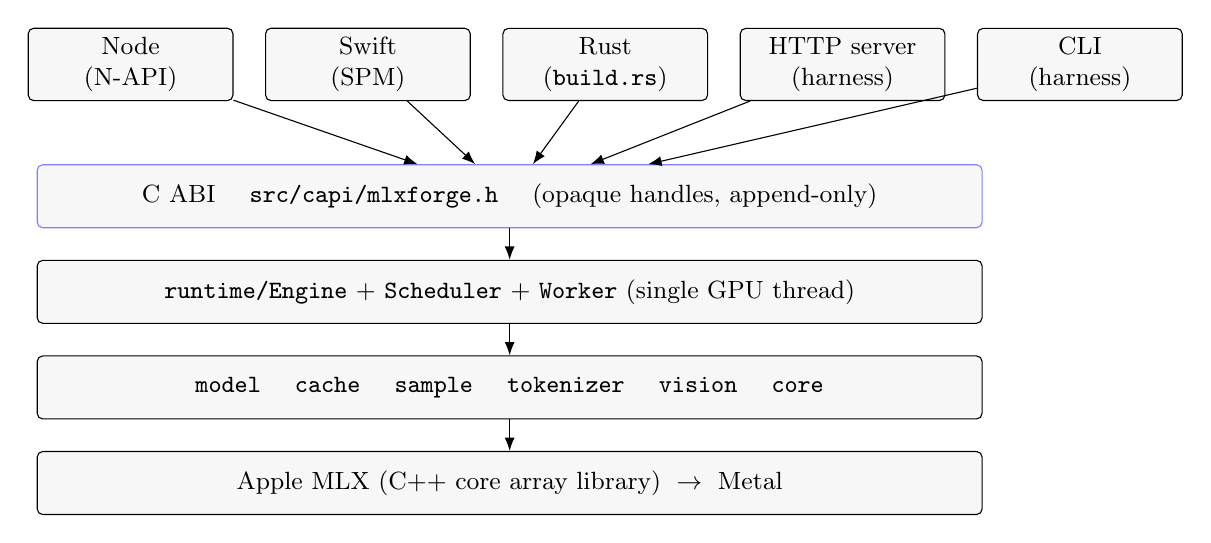
\begin{tikzpicture}[
  font=\small,
  box/.style={draw,rounded corners=2pt,minimum height=8mm,minimum width=26mm,align=center,fill=black!3},
  wide/.style={box,minimum width=120mm},
  prod/.style={box,fill=blue!8,draw=blue!50},
  node distance=4mm,
]
  \node[box] (node)  {Node\\(N-API)};
  \node[box,right=of node] (swift) {Swift\\(SPM)};
  \node[box,right=of swift] (rust) {Rust\\(\code{build.rs})};
  \node[box,right=of rust] (srv) {HTTP server\\(harness)};
  \node[box,right=of srv] (cli) {CLI\\(harness)};

  \node[prod,wide,below=8mm of swift,xshift=18mm] (abi) {C ABI \quad \code{src/capi/mlxforge.h} \quad (opaque handles, append-only)};

  \node[wide,below=of abi] (engine) {\code{runtime/Engine} + \code{Scheduler} + \code{Worker} (single GPU thread)};
  \node[wide,below=of engine] (core) {\code{model} \quad \code{cache} \quad \code{sample} \quad \code{tokenizer} \quad \code{vision} \quad \code{core}};
  \node[wide,below=of core] (mlx) {Apple MLX (C++ core array library) \;$\rightarrow$\; Metal};

  \foreach \a in {node,swift,rust,srv,cli} { \draw[-{Latex}] (\a) -- (abi); }
  \draw[-{Latex}] (abi) -- (engine);
  \draw[-{Latex}] (engine) -- (core);
  \draw[-{Latex}] (core) -- (mlx);
\end{tikzpicture}
\caption{Layered architecture. The stable C ABI is the product boundary; bindings
and the server/CLI harnesses are consumers above it.}
\label{fig:layers}
\end{figure}

\section{Build products and dependencies}
\code{mlxforge\_core} is a static library aggregating all modules. Three products
build on top of it: \code{libmlxforge} (the C-ABI shared library, which is the
product), the \code{mlxforge} server, and the \code{mlxforge-cli} tool. The server and CLI
are gated behind build flags so the released library is lean:

\begin{lstlisting}[language=none,caption={Lean library build (no httplib, no curl).}]
cmake -S . -B build \
  -DMLXFORGE_BUILD_SERVER=OFF \
  -DMLXFORGE_BUILD_CLI=OFF \
  -DMLXFORGE_ENABLE_HF_DOWNLOAD=OFF
\end{lstlisting}

Dependencies are pinned in \code{cmake/Dependencies.cmake}: MLX v0.31.2,
cpp-httplib (server only), doctest (tests), spdlog v1.15.3, \code{stb\_image}
(vision, header-only), and \code{nlohmann/json} transitively from MLX. System
\code{libcurl} is found via \code{find\_package(CURL)} and linked privately, only
for HuggingFace downloads.

\section{Model-source resolution}
The CLI and server take a model \emph{spec}, either a local directory or a
HuggingFace repo id, and resolve it once via
\code{mlxforge::resolve\_model\_dir} (\code{src/core/model\_source}). Resolution
walks a five-tier hierarchy:
\begin{enumerate}[nosep]
  \item an existing local directory with \code{config.json} is used as-is;
  \item an existing HF parent directory (\code{models--org--name}) is resolved to
        its \code{snapshots/<rev>/};
  \item a repo already in the standard HF hub cache is reused;
  \item a repo already downloaded by \code{mlxforge} is reused;
  \item otherwise it is downloaded (via \code{libcurl}, the only HTTP \emph{client}
        in the tree) into \code{\$MLXFORGE\_CACHE} (default
        \code{\textasciitilde/.cache/mlxforge}).
\end{enumerate}

% ===========================================================================
\chapter{Threading Model and the Single-Worker Invariant}
\label{ch:threading}

\section{One fact drives the whole design}
MLX is not thread-safe, and MLX arrays are thread-bound: GPU work must run on the
thread that created the arrays. The entire concurrency architecture falls out of
this single fact.

\begin{quote}
\emph{Exactly one GPU worker thread loads the model on itself and is the only
thread that ever calls \code{mx::eval} or \code{mx::async\_eval}.}
\end{quote}

Every other thread (HTTP request threads from the server's pool, test threads,
binding callers) touches only its own \code{Request} struct and the thread-safe
\code{Scheduler} queue. Because there is exactly one place MLX runs, there is
nothing to contend over. No GPU-state mutex, no reader/writer locks, no
compare-and-swap on model state. Concurrency correctness comes from the structure
itself, not from locking the GPU.

\begin{table}[h]
\centering
\caption{Thread roles.}
\label{tab:threads}
\small
\begin{tabular}{@{}l p{0.42\linewidth} p{0.30\linewidth}@{}}
\toprule
Thread & Responsibility & Constraint \\
\midrule
GPU worker        & Model load, forward passes, sampling, KV cache, scheduler loop
                  & Only MLX caller; loads model on itself \\
Request threads   & Parse, chat template, tokenize, submit, stream out
                  & Never call MLX; touch only own \code{Request} \\
Test/binding threads & Drive concurrent requests
                  & Submit, wait on token queue \\
\bottomrule
\end{tabular}
\end{table}

\section{The request lifecycle}
A request passes through four phases (Figure~\ref{fig:flow}):

\begin{enumerate}[nosep]
  \item \textbf{Submit} (any thread). Parse the request body, render the chat
        template, tokenize. Build a \code{Request} carrying prompt ids, sampling
        parameters, \code{max\_tokens}, EOS ids, a bounded token queue, and a
        \code{cancelled} atomic. \code{Scheduler::submit()} pushes it onto the
        waiting deque and notifies the worker. If the waiting queue is full,
        submission fails (the server replies \code{429}).
  \item \textbf{Admit / Prefill} (worker). Drain up to a fixed number of waiting
        requests, left-pad their prompts to a common length, run a dedicated
        prefill forward (chunked to bound memory), merge the prefilled K/V into the
        persistent decode cache, and sample each row's first token.
  \item \textbf{Decode} (worker, steady state). Each loop iteration runs exactly
        one batched decode step over all active rows.
  \item \textbf{Evict} (worker). A row finishes on EOS
        (\code{finish\_reason="stop"}), on \code{max\_tokens}
        (\code{"length"}), or on client disconnect (\code{"cancel"}). Finished
        rows are dropped from the cache and their token queue is closed; freed
        slots are filled by admitting more waiting requests.
\end{enumerate}

\begin{figure}[t]
\centering
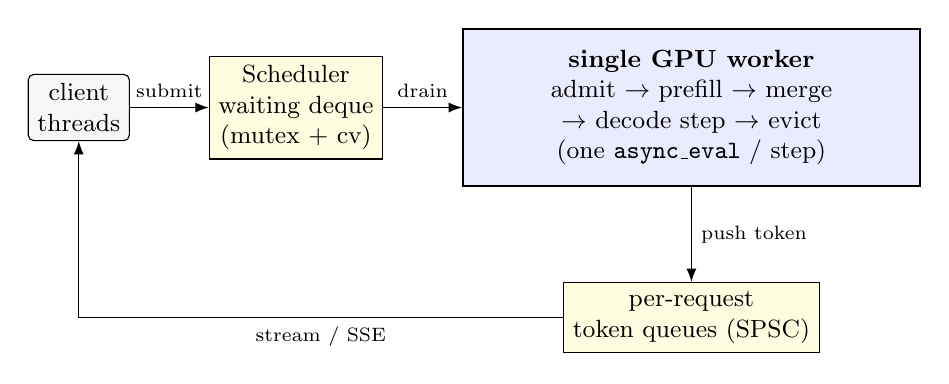
\begin{tikzpicture}[
  font=\small,
  node distance=6mm and 10mm,
  io/.style={draw,rounded corners=2pt,align=center,fill=black!3,minimum height=8mm},
  q/.style={draw,align=center,fill=yellow!12,minimum height=8mm},
  w/.style={draw,thick,align=center,fill=blue!8,minimum width=58mm,minimum height=20mm},
]
  \node[io] (client) {client\\threads};
  \node[q,right=of client] (wait) {Scheduler\\waiting deque\\(mutex + cv)};
  \node[w,right=of wait] (worker) {\textbf{single GPU worker}\\admit $\rightarrow$ prefill $\rightarrow$ merge\\$\rightarrow$ decode step $\rightarrow$ evict\\(one \code{async\_eval} / step)};
  \node[q,below=12mm of worker] (tq) {per-request\\token queues (SPSC)};

  \draw[-{Latex}] (client) -- node[above,font=\scriptsize]{submit} (wait);
  \draw[-{Latex}] (wait) -- node[above,font=\scriptsize]{drain} (worker);
  \draw[-{Latex}] (worker) -- node[right,font=\scriptsize]{push token} (tq);
  \draw[-{Latex}] (tq) -| node[below,font=\scriptsize,pos=0.25]{stream / SSE} (client);
\end{tikzpicture}
\caption{Request flow. Client threads only ever push to the waiting queue and pop
from their own token queue; the worker exclusively owns all MLX state.}
\label{fig:flow}
\end{figure}

\section{Producer/consumer handoff and backpressure}
Each request carries a bounded, blocking single-producer/single-consumer queue
(\code{SpscQueue}). The worker is the sole producer; the request thread is the sole
consumer. Bounding the queue gives backpressure for free: a slow streaming client
cannot make the worker accumulate unbounded tokens, because \code{push} blocks once
the queue is full. Cancellation is an atomic flag the worker checks at iteration
boundaries, so a disconnected client gets evicted right away.

% ===========================================================================
\chapter{Continuous-Batching Scheduler}
\label{ch:batching}

\section{Goals}
The scheduler has four jobs. It serves concurrent users on one GPU worker, admits
new work into an active batch and evicts finished work dynamically, keeps one GPU
graph alive rather than recompiling per request, and (the highest-severity
invariant) issues exactly one \code{async\_eval} per decode step covering the whole
batch. The design follows the continuous-batching lineage of Orca~\citep{yu2022orca} and
vLLM~\citep{kwon2023vllm}, adapted to MLX's lazy-graph execution and the absence of
a paged-attention primitive.

\section{Prefill as a separate pass}
Prefill and decode have different tensor shapes: prefill processes
$(B_{\text{pre}}, P_{\max})$ tokens, decode processes $(B_{\text{dec}}, 1)$.
Rather than interleave them, prefill is a distinct pass. All prompts in a prefill
batch are \emph{left-padded} to a common length $P_{\max}$ so that every row's last
real token lands at the same physical column, which lines up the handoff into
decode. Long prompts are chunked (in steps of 2048 tokens), evaluating cache state
at chunk boundaries to bound graph and memory growth. The prefilled K/V is then
merged into the live decode cache.

\section{The one-eval-per-step invariant}
In steady-state decode, each iteration of the worker loop:
\begin{enumerate}[nosep]
  \item gathers the next input token per row into an $(B,1)$ array;
  \item computes \code{logits = model.forward(inputs, cache)}, an $(B,1,V)$ tensor,
        with each row's RoPE position read from the cache and a ragged additive
        mask built so left-padded rows attend only their own history;
  \item samples the next token per row;
  \item issues \emph{one} \code{mx::async\_eval} for the entire batch this step,
        never per row and never per layer;
  \item reads the chosen ids back to the host and pushes each row's token.
\end{enumerate}
This is the single most important performance and correctness rule in the engine.
\code{Worker::decode\_steps()} counts these evaluations, and under load the step
count sits far below the total token count. That gap is the operational proof that
batching is actually happening.

\section{Batch-size bucketing}
A varying batch size would force MLX to re-trace and re-compile the decode graph
each time the population changes. To avoid this, the active batch size is rounded up
to a fixed bucket in $\{1,2,4,8,16,32,64,128,\dots\}$ by appending masked dummy
rows (\code{BatchKVCache::pad\_dummies}). Dummy rows attend only to their own
position, contributing nothing, and are trimmed back with \code{filter()} after the
step. The GPU graph shape stays stable across admit/evict churn.

\section{Memory admission gate}
Before admitting a batch, the worker projects its peak KV footprint. For an fp16
cache,
\begin{equation}
  \text{bytes per token} = 2 \cdot n_{\text{layers}} \cdot n_{\text{kv\,heads}}
  \cdot d_{\text{head}} \cdot \mathrm{sizeof}(\text{fp16}),
\end{equation}
where the factor 2 accounts for keys and values. For Llama-3.2-1B
($n_{\text{layers}}=16$, $n_{\text{kv\,heads}}=8$, $d_{\text{head}}=64$) this is
$2\cdot16\cdot8\cdot64\cdot2 = 32{,}768$ bytes ($32$\,KiB) per token. Under KV-cache
quantization (Section~\ref{sec:kvquant}) the per-head row cost changes to
$d\cdot b/8$ packed bytes plus an fp16 scale and bias per group: with $d=64$ and
group size 64, 68 bytes at 8-bit and 36 bytes at 4-bit versus 128 bytes fp16,
and the budget projection accounts for it. A batch whose
projected footprint would exceed the configured budget
(\code{src/cache/kv\_budget}) is refused. Together with the bounded waiting queue
(which returns \code{429} on overflow), this keeps the engine from running out of
memory under load.

% ===========================================================================
\chapter{The Transformer Forward Pass}
\label{ch:forward}

This chapter documents the dense decoder forward pass implemented by
\code{DecoderModel} (\code{src/model/decoder\_model.cpp}), the base class for every
supported family. Equations are written to match the code, which in turn matches
the \code{mlx-lm} reference.

\section{Notation}
Let $B$ be batch size, $L$ the sequence length of the current step, $H$ the hidden
size, $n_h$ the number of query heads, $n_{kv}$ the number of key/value heads,
$d=d_{\text{head}}$ the per-head dimension (so $H = n_h d$), and $V$ the vocabulary
size. A linear layer with HuggingFace weight $W \in \R^{\text{out}\times\text{in}}$
computes $xW^\top$; the code stores weights as $(\text{out},\text{in})$ and
transposes, so forgetting the transpose is a silent bug.

\section{Embedding}
Token ids index rows of the embedding matrix
$E \in \R^{V\times H}$:
\begin{equation}
  h^{(0)}_{b,\ell} = E_{\,t_{b,\ell}}, \qquad h^{(0)} \in \R^{B\times L\times H}.
\end{equation}
For a quantized checkpoint, only the gathered rows are dequantized
(Chapter~\ref{ch:quant}), so the full fp16 embedding table is never materialized.

\section{RMSNorm}
Every normalization is RMSNorm~\citep{zhang2019rmsnorm}, with a learned gain $w$ and
$\varepsilon$ from the config:
\begin{equation}
  \rmsnorm(x, w) = w \elemmul \frac{x}{\sqrt{\frac{1}{H}\sum_{i=1}^{H} x_i^2 + \varepsilon}}.
\end{equation}
It is applied before attention (\code{input\_layernorm}), before the MLP
(\code{post\_attention\_layernorm}), and once more before the LM head
(\code{model.norm}).

\section{Grouped-query attention}
\label{sec:gqa}
For layer $\ell$, the normalized input is projected to queries, keys, and values:
\begin{align}
  Q &= \text{reshape}\big(\rmsnorm(h, w^{\text{in}}_\ell)\,W^Q_\ell\big) \in \R^{B\times n_h\times L\times d},\\
  K &= \text{reshape}\big(\rmsnorm(h, w^{\text{in}}_\ell)\,W^K_\ell\big) \in \R^{B\times n_{kv}\times L\times d},\\
  V &= \text{reshape}\big(\rmsnorm(h, w^{\text{in}}_\ell)\,W^V_\ell\big) \in \R^{B\times n_{kv}\times L\times d}.
\end{align}
With $n_{kv} < n_h$ this is grouped-query attention~\citep{ainslie2023gqa}; the head
repeat is handled \emph{natively} by MLX's scaled dot-product attention (SDPA).
Manually repeating heads instead produces a subtly different token sequence and is a
known silent-bug source. Optionally a per-head normalization hook
$\code{norm\_qk\_head}$ is applied to $Q$ and $K$ (identity for Llama, RMSNorm over
$d$ for Qwen3) before RoPE. After applying RoPE (Chapter~\ref{ch:rope}) and updating
the cache, attention is
\begin{equation}
  \text{Attn}(Q,K,V) = \softmax\!\left(\frac{QK^\top}{\sqrt{d}} + M\right)V,
\end{equation}
where the softmax is computed in fp32 internally. During multi-token prefill the
mask $M$ is causal; for a single decode token over cached history it is empty
(unmasked); for the batched decode path it is the explicit additive mask of
Chapter~\ref{ch:mask}. The output is reshaped back to $\R^{B\times L\times H}$ and
passed through the output projection $W^O_\ell$.

\section{SwiGLU feed-forward}
The dense MLP is a SwiGLU~\citep{shazeer2020glu} block with gate, up, and down
projections and the SiLU activation $\silu(z) = z\,\sigma(z)$:
\begin{equation}
  \text{MLP}(x) = \Big(\silu(x\,W^{\text{gate}}) \elemmul (x\,W^{\text{up}})\Big) W^{\text{down}}.
\end{equation}

\section{The decoder block and the head}
Each block applies attention and MLP with residual connections, and a post-attention
norm between them:
\begin{align}
  h' &= h + \text{Attn-sublayer}(\rmsnorm(h, w^{\text{in}}_\ell)),\\
  h'' &= h' + \text{MLP}\big(\rmsnorm(h', w^{\text{post}}_\ell)\big).
\end{align}
After $n_{\text{layers}}$ blocks, a final RMSNorm and the LM head produce logits:
\begin{equation}
  \text{logits} = \rmsnorm(h, w^{\text{norm}})\, W_{\text{lm}}^\top \in \R^{B\times L\times V},
\end{equation}
where $W_{\text{lm}}$ is either a separate \code{lm\_head.weight} or the tied
embedding matrix $E$, depending on the checkpoint.

\section{Family extension via virtual hooks}
\code{DecoderModel} is the shared base; model families override a small set of
virtual hooks rather than duplicating the forward pass
(Table~\ref{tab:hooks}). This is the strategy/template-method pattern applied to a
numerical kernel.

\begin{table}[h]
\centering
\caption{Virtual hooks on \code{DecoderModel} and their family overrides.}
\label{tab:hooks}
\small
\begin{tabular}{@{}l p{0.62\linewidth}@{}}
\toprule
Hook & Override \\
\midrule
\code{norm\_qk\_head} & Identity (Llama); RMSNorm over $d$ before RoPE (Qwen3). \\
\code{feed\_forward}  & Dense SwiGLU; sparse MoE routing (Qwen3 MoE). \\
\code{decoder\_block} & Attention+MLP; hybrid attention/linear routing (Qwen3.5). \\
\code{attention}      & Standard GQA; gated + partial-RoPE attention (Qwen3.5). \\
\bottomrule
\end{tabular}
\end{table}

% ===========================================================================
\chapter{Rotary Position Embeddings}
\label{ch:rope}

\section{Base frequencies}
RoPE~\citep{su2021rope} rotates pairs of channels by an angle proportional to
position. The per-channel inverse frequencies, for the even indices
$i=0,2,\dots,d-2$, are
\begin{equation}
  \theta_i = \text{base}^{\,-\,i/d}, \qquad \text{base} = \texttt{rope\_theta},
\end{equation}
giving $d/2$ values. The code computes this as
$\text{base}^{\,\text{arange}(0,d,2)/d}$ and feeds the reciprocals (via
\code{fast::rope}). A token at position $m$ rotates channel pair $i$ by $m\theta_i$:
\begin{equation}
  \rope(x, m)_{[2i,2i+1]} =
  \begin{pmatrix} \cos m\theta_i & -\sin m\theta_i \\ \sin m\theta_i & \cos m\theta_i \end{pmatrix}
  \begin{pmatrix} x_{2i} \\ x_{2i+1} \end{pmatrix}.
\end{equation}

\section{Llama-3 frequency rescaling}
Llama-3 rescales these frequencies to extend context, and \code{mlxforge} mirrors
\code{mlx-lm}'s \code{Llama3RoPE} exactly (validated against the
\code{rope\_freqs.npy} fixture). Let $f$ be the scaling \code{factor}, $\beta_{lo}$
and $\beta_{hi}$ the low/high frequency factors, and $C$ the original context
length. Define the wavelength of channel $i$ as $\lambda_i = 2\pi/\theta_i$ (the
code uses $\lambda_i = 2\pi\theta_i$ on the reciprocal-frequency representation; the
banding is identical). With wavelength thresholds
$\lambda_{lo} = C/\beta_{lo}$ and $\lambda_{hi} = C/\beta_{hi}$, the rescaled
frequency is piecewise:
\begin{equation}
  \theta_i' =
  \begin{cases}
    \theta_i / f & \lambda_i > \lambda_{lo} \quad (\text{low frequency}),\\[4pt]
    \dfrac{\theta_i}{(1-s_i)/f + s_i} & \lambda_{hi} < \lambda_i < \lambda_{lo} \quad (\text{medium}),\\[10pt]
    \theta_i & \text{otherwise} \quad (\text{high frequency}),
  \end{cases}
\end{equation}
where the smooth interpolation factor is
\begin{equation}
  s_i = \frac{C/\lambda_i - \beta_{lo}}{\beta_{hi} - \beta_{lo}}.
\end{equation}
Low-frequency (long-wavelength) channels are stretched by $f$, high-frequency
channels are untouched, and a smooth blend bridges the band between. GGUF
checkpoints bake this rescaling into a per-dimension factor array
$\texttt{rope\_freq\_factors}$, so the engine just multiplies:
$\theta_i' = \text{base}^{-i/d}\cdot \texttt{factors}_i$.

\section{Batched application with per-row offset}
\code{fast::rope} takes either a scalar offset (prefill) or a per-row offset array
(batched decode). The latter is essential: in a continuous batch, each row sits at a
different position in its own sequence, so RoPE must rotate each row by its own
$m$. The precomputed (and possibly rescaled) frequencies are passed directly; the
base is disabled so the rescaling is not applied twice. The math is not
``simplified'' in code precisely because any deviation is silent.

% ===========================================================================
\chapter{Attention Masking}
\label{ch:mask}

\section{Additive fp16, never boolean}
All masks are additive fp16 tensors, never boolean. Boolean masks trigger MLX issue
\#2894, so the engine adds $0$ to kept positions and $-\infty$ to masked ones:
\begin{equation}
  M_{b,q,k} =
  \begin{cases} 0 & \text{keep},\\ -\infty & \text{mask}. \end{cases}
\end{equation}

\section{The batched decode mask}
For the continuous-batching path, the mask must encode both causality and per-row
left-padding simultaneously. Let \code{prev\_idx} be the populated cache length
before this step, $N$ the number of query tokens, and $\ell_b$ the left-padding of
row $b$. With key positions $k \in [0, T_{kv})$ where $T_{kv}=\code{prev\_idx}+N$,
and query positions $q \in [\code{prev\_idx},\, \code{prev\_idx}+N)$, the keep
predicate is
\begin{equation}
  \text{keep}_{b,q,k} = \underbrace{[\,q \ge k\,]}_{\text{causal}} \;\wedge\; \underbrace{[\,\ell_b \le k\,]}_{\text{not padding}},
\end{equation}
producing a $\R^{B\times 1\times N\times T_{kv}}$ additive mask. The mask therefore
operates in \emph{physical-slot space} (indices into the contiguous cache),
dropping the left-pad region while preserving causal order. This decoupling (mask
in slot space, RoPE in logical-position space) is what lets a left-padded ragged
batch share one contiguous cache (Chapter~\ref{ch:cache}).

% ===========================================================================
\chapter{KV Cache}
\label{ch:cache}

\section{Single-sequence cache}
\code{KVCache} (\code{src/cache/kv\_cache}) holds per-layer key/value arrays and a
scalar offset. \code{update\_and\_fetch} concatenates the new step's K/V onto the
sequence axis and returns the accumulated K/V of shape
$(1, n_{kv}, \text{seq}, d)$. It also carries optional convolution and recurrent
state for the Qwen3.5 linear-attention layers (Chapter~\ref{ch:families}).

\section{Batched cache: left-padded and contiguous}
\code{BatchKVCache} (\code{src/cache/batch\_kv\_cache}) is the data structure that
serves both efficiency and multi-user serving. It is \emph{left-padded and
contiguous}, not paged: MLX's C++ surface has no paged-attention primitive, and SDPA
wants contiguous K/V. At the $\sim$1B parameter scale the padding waste is
acceptable, and the contiguous layout keeps the kernel simple. (Prefix sharing is
layered on top through a block pool rather than through paging; see
Section~\ref{sec:prefixcache}.) The cache tracks:
\begin{itemize}[nosep]
  \item \code{idx}: the populated sequence length (physical write position);
  \item \code{offset}: a per-row $(B,)$ RoPE position, which can differ from
        \code{idx} (used for vision prefill, below);
  \item \code{left\_padding}: a per-row $(B,)$ count of leading pad slots.
\end{itemize}
Capacity grows in blocks of 256 tokens to amortize reallocation. The valid key range
for row $b$ is the slot interval $[\ell_b, \code{idx})$.

\section{Decoupling RoPE position from physical length}
The key design move is that \code{offset} (logical RoPE position) is separate from
\code{idx}/\code{left\_padding} (physical slots). \code{from\_single\_sequence}
exploits this: after a Qwen3-VL vision prefill, where image patches collapse many
tokens into few \emph{positions}, the batch-1 cache is created with
\code{idx} equal to the physical token count but \code{offset} equal to the maximum
3D M-RoPE position (which is smaller). A generated VL token is pure text, so it
decodes through the ordinary batched forward, carrying
$\code{offset} = \max(\text{3D position}) + 1$, well below its image-padded token
count, and no per-row 3D positions are needed in the cache.

\section{Batch surgery}
Three operations reshape the batch as it churns:
\begin{itemize}[nosep]
  \item \code{filter(keep)} retains selected rows (eviction), then shifts off
        any common left-padding shared by all survivors;
  \item \code{merge(other)} right-justifies two caches to a common length and
        capacity and concatenates on the batch axis (admission of a freshly
        prefilled batch);
  \item \code{pad\_dummies(extra)} appends masked dummy rows for bucketing
        (Chapter~\ref{ch:batching}).
\end{itemize}

\section{Quantized KV storage}
\label{sec:kvquant}
The engine option \code{kv\_bits} (default 0, i.e.\ dense fp16; 8 or 4 to enable)
stores the KV cache quantized, cutting its memory by $\sim$1.9$\times$ at 8-bit
(near-lossless) or $\sim$3.6$\times$ at 4-bit. The implementation
(\code{src/cache/kv\_quant}) deliberately mirrors \code{mlx-lm}'s
\code{QuantizedKVCache}:

\begin{itemize}[nosep]
  \item \textbf{Triplet storage, quantized at write time.} Each cached K or V
        tensor is the 3-tuple \code{mx::quantize} produces: packed
        \code{uint32} words plus per-group fp16 scales and biases (group size 64,
        which must divide $d$). Quantization happens per position as tokens are
        written, so prefill chunking can never change the stored values. Both
        \code{KVCache} and \code{BatchKVCache} hold per-layer \emph{component
        vectors} (one array dense, three quantized); all batch surgery
        (\code{filter}/\code{merge}/\code{pad\_dummies}, block growth) runs per
        component unchanged.
  \item \textbf{Hand-rolled quantized attention.} MLX has no fused quantized SDPA
        kernel, so \code{quantized\_sdpa} (\code{src/model/sdpa}) ports
        \code{mlx\_lm/models/base.py} op-for-op: \code{quantized\_matmul} for the
        scores and the output, GQA via a $(B, n_{kv}, n_{\text{rep}}, L, d)$
        reshape, precise softmax. \code{sdpa\_with\_cache} is the dispatch seam
        every model attention call site uses, selecting the dense fast kernel or
        the quantized path by the cache's configuration.
  \item \textbf{Engine-wide scope, no silent fallback.} The batched cache's
        storage is physically shared across rows, so the setting cannot be
        per-request. Unsupported setups (vision-language and hybrid Qwen3.5
        models, which have no quantized golden reference yet; group sizes that do
        not divide $d$) fail engine creation rather than falling back to fp16.
\end{itemize}

Three numerical traps shaped the implementation. First, under GQA the batched
additive mask must be reshaped $(B,1,N,T)\to(B,1,1,N,T)$, and masked columns
must be \emph{overridden} with $\min(\text{fp16})$, never added: a fully-masked
left-pad row produces NaN that adding $-\infty$ cannot cancel. Second, quantized
matmuls are \emph{fusion-context-sensitive}: the same matmul shifts by $\sim$1
logit between lazy and materialized inputs, and \code{mlx-lm} disagrees with
itself across graph contexts, so bit-exact cross-implementation gating is
unsound. The golden gates are therefore teacher-forced and \emph{margin-gated}:
token equality is asserted at every step whose reference top-2 logit margin
clears the fusion-context noise, plus an exact batched-versus-single-stream
coherence gate. Third, both caches share the block-grow $+$
\code{slice\_update} storage writer (\code{update\_kv\_components}) because
buffer shapes and strides affect kernel accumulation order; the exact-token
gates depend on the layouts matching \code{mlx-lm} bit-for-bit.

\section{Prefix cache: block-pool KV storage}
\label{sec:prefixcache}
The engine option \code{prefix\_cache} (default off) reuses K/V across requests
that share a token prefix --- the shared-system-prompt and multi-turn
conversation shapes. On a 2048-token shared prefix the warm time-to-first-token
drops $\sim$20$\times$ (measured by \code{mlxforge-cli bench-prefix}); decode
throughput is unchanged.

The design is \emph{gather-on-admit, not paged attention}. vLLM's
PagedAttention~\citep{kwon2023vllm} runs attention directly over scattered
pages, but MLX has no paged SDPA kernel and \code{mlx-lm} has no paged reference
to gate one against, so the decode batch stays the contiguous left-padded
\code{BatchKVCache} of this chapter. The \emph{pages} live in a pool instead,
and matched pages are copied into a row's cache on admission --- cheap under
Apple Silicon's unified memory next to the prefill they replace.

\begin{itemize}[nosep]
  \item \textbf{Block pool.} \code{BlockPool} (\code{src/cache/block\_pool})
        holds immutable \code{KVBlock}s of \code{kv\_block\_size} tokens (default
        256; all layers, the same dense or quantized component vectors the caches
        store), LRU-evicted under a configurable byte budget. Each block is keyed
        by a \emph{chain hash}: an FNV-1a-64 hash of the block's own token ids
        chained onto the previous block's key, so a key identifies the
        \emph{entire} token prefix up to the block's end --- two prompts share a
        block only if they share every token before it. Keys are salted with the
        model fingerprint and storage configuration, so a persisted block can
        never cross models or quantization settings.
  \item \textbf{Matching and admission.} \code{PrefixCache}
        (\code{src/cache/prefix\_cache}) matches a prompt to its longest chain of
        consecutive cached full blocks, clamped to $\text{prompt\_len}-1$ tokens
        so the admission still produces next-token logits (the last prompt token
        is always recomputed --- the same rule vLLM and
        SGLang~\citep{zheng2024sglang} use). Matched blocks seed a batch-1 cache
        via \code{BatchKVCache::from\_prefix}, written through the standard
        block-grow storage writer so the buffer layout matches a cold prefill
        (strides are load-bearing, per Section~\ref{sec:kvquant}); only the
        suffix is prefilled, and the row then merges into the decode batch like
        any single-row admission.
  \item \textbf{Harvest is prompt-only.} When a row finishes, only its
        \emph{prompt} span is sealed into the pool --- never decode-produced K/V.
        Decode-with-cache K/V differs from a recompute by fp16 accumulation order
        (the decode-versus-recompute gap of Chapter~\ref{ch:testing}) and
        demonstrably flips later greedy choices; prefill-produced K/V is the
        proven exact-stable class, so pooling only it keeps the feature's gate
        (warm $=$ cold, token-exact) sound. Multi-turn reuse still converges:
        the next turn's prompt contains the prior answer as text, so its
        (prefix-seeded) prefill recomputes that span once and pools it. Harvested
        slices are materialized (\code{mx::contiguous} $+$ eval) so the pool
        never pins the batch cache's buffers, and multimodal rows are never
        harvested or matched (a token-id hash cannot identify image content or
        3D positions).
\end{itemize}

Like \code{kv\_bits}, the setting is engine-wide (the pool stores one storage
layout), and hybrid and vision-language models reject it at engine creation.

\section{SSD spill tier}
\label{sec:spill}
An optional spill directory (\code{kv\_spill\_dir}) adds a second cache level
under the RAM pool (\code{src/cache/block\_store}). Blocks LRU-evicted from RAM
are serialized and written as one file per block (\code{<hash>.kvb},
created \code{0600} since the cache holds conversation content, written
tmp-then-rename); a pool miss revives the file synchronously --- an SSD read of
a few megabytes replaces a far more expensive prefill. The directory is
rescanned at construction, so the prefix cache survives engine restarts, and an
on-disk byte budget LRU-deletes files beyond it.

The threading split follows the thread-bound-arrays rule
(Chapter~\ref{ch:threading}): \code{BlockStore} itself never touches MLX arrays
--- its asynchronous writer thread and file index handle only raw byte buffers,
while the array$\leftrightarrow$bytes conversions run on the worker thread,
which owns every pooled array. The writer keeps a queued block visible to
\code{get()}/\code{contains()} until its file lands. The versioned on-disk
format embeds the salt, verified on load (any mismatch or truncation is treated
as a plain miss), and its serialize order --- per layer, K components then V ---
is gated by an exact-token spill test, because an order mismatch produced
silent garbage.

% ===========================================================================
\chapter{Sampling and Constrained Decoding}
\label{ch:sampling}

The sampler (\code{src/sample/sampler.cpp}) expresses every operation as an MLX
graph op over the logits, so it folds into the single per-step \code{async\_eval};
no values leave the GPU mid-pipeline.

\section{Greedy and temperature}
Greedy decoding is $\arg\max$ over the vocabulary. Otherwise logits are scaled by
temperature $\tau$: $z' = z/\tau$. As $\tau\to 0$ this degenerates to greedy; $\tau>1$
flattens the distribution.

\section{Truncation filters}
Three filters truncate the candidate set before the categorical draw:
\begin{itemize}[nosep]
  \item \textbf{Top-$k$}: keep the $k$ largest logits, set the rest to $-\infty$.
  \item \textbf{Top-$p$ (nucleus)}~\citep{holtzman2020nucleus}: sort descending,
        form the softmax, and keep the smallest prefix whose \emph{prior} cumulative
        mass is below $p$:
        \begin{equation}
          \text{keep token } j \iff \sum_{r < j} p_{(r)} < p,
        \end{equation}
        then restore vocabulary order.
  \item \textbf{Min-$p$}: keep tokens with probability at least $p_{\min}$ times the
        peak probability: $p_j \ge p_{\min}\cdot \max_i p_i$.
\end{itemize}

\section{Penalties}
Given the token history, three penalties reshape the logits:
\begin{align}
  \text{repetition:}\quad & z_j \leftarrow z_j/\rho \text{ if } z_j>0,\ \text{else } z_j\cdot\rho, \quad \text{for seen } j;\\
  \text{frequency:}\quad  & z_j \leftarrow z_j - c_j\,\alpha_{\text{freq}}, \quad c_j = \text{count of } j \text{ in history};\\
  \text{presence:}\quad   & z_j \leftarrow z_j - \mathbb{1}[c_j>0]\,\alpha_{\text{pres}}.
\end{align}

\section{Log-probabilities}
When requested (OpenAI \code{logprobs}/\code{top\_logprobs}), the engine reports the
log-probability of the chosen token and of the top-$k$ alternatives. These are
computed from the \emph{penalized but pre-filter} distribution (a coherent softmax
over the full vocabulary), not from the temperature-scaled, truncated logits, so
they are well-defined probabilities.

\section{Constrained JSON decoding}
For structured output, a JSON grammar engine (\code{src/sample/json\_grammar.cpp})
masks the logits each step so only tokens that keep the output a valid prefix of the
target schema survive. The grammar engine is pure and unit-tested; its cost is an
opt-in per-step host-side vocabulary scan.

% ===========================================================================
\chapter{Model Families}
\label{ch:families}

Table~\ref{tab:families} summarizes the per-family deltas over the dense Llama base.

\begin{table}[h]
\centering
\caption{Model families and their deltas.}
\label{tab:families}
\small
\begin{tabular}{@{}l p{0.58\linewidth} l@{}}
\toprule
Family & Delta over dense Llama & Status \\
\midrule
Llama-3.2     & base case                                        & fp16/4-bit/GGUF \\
Qwen3 dense   & per-head QK-Norm; ChatML template                & fp16/4-bit/GGUF \\
Qwen3 MoE     & sparse mixture-of-experts FFN                    & fp16/4-bit/GGUF \\
Qwen3.5 hybrid& gated full attn + Gated-DeltaNet linear attn     & 4-bit (text) \\
Qwen3-VL      & ViT + image merge + 3D M-RoPE + DeepStack        & 4-bit (vision) \\
\bottomrule
\end{tabular}
\end{table}

\section{Qwen3 dense}
Qwen3 adds RMSNorm over the head dimension to $Q$ and $K$ before RoPE (the
\code{norm\_qk\_head} hook) and uses the ChatML chat template. Everything else is the
dense base.

\section{Qwen3 MoE}
A sparse layer replaces the dense MLP with a router and a pool of experts
(\code{src/model/qwen3\_moe.cpp}), following the sparse-MoE
lineage~\citep{fedus2022switch,jiang2024mixtral}. The router produces a distribution
over $E$ experts (fp32 softmax to match the reference), the top $k$ experts are
selected, their scores optionally renormalized, and the outputs combined:
\begin{equation}
  g = \softmax(x\,W^{\text{router}}), \qquad
  \mathcal{T} = \operatorname{top\text{-}k}(g), \qquad
  \alpha_e = \frac{g_e}{\sum_{e'\in\mathcal{T}} g_{e'}}\ (e\in\mathcal{T}),
\end{equation}
\begin{equation}
  y = \sum_{e\in\mathcal{T}} \alpha_e \cdot \text{SwiGLU}_e(x).
\end{equation}
Top-$k$ uses \code{argpartition} (the intra-$k$ order is irrelevant since outputs are
summed). Per-expert projections are computed with a gather matmul
(\code{gather\_mm}, or \code{gather\_qmm} when quantized) so only each token's
selected experts are evaluated. A checkpoint may mix precisions (e.g.\ an 8-bit
router with 4-bit experts); per-weight quantization detection handles this
transparently.

\section{Qwen3.5 hybrid}
Qwen3.5 interleaves two layer types (routed by
$\code{is\_linear\_layer}(\ell)$): gated full-attention layers and Gated-DeltaNet
linear-attention layers~\citep{yang2024gateddeltanet}.

\paragraph{Partial RoPE and output gating.} The full-attention layers apply RoPE to
only the leading $\lfloor d\cdot\texttt{partial\_rotary\_factor}\rfloor$ channels,
leaving the tail un-rotated. The query projection is double-width, producing queries
and a gate; the attention output is elementwise-scaled by $\sigma(\text{gate})$
before the output projection.

\paragraph{Gated-DeltaNet recurrence.} The linear-attention layer maintains a
fixed-size recurrent state $S_t \in \R^{H_v\times D_v\times D_k}$ (accumulated in
fp32 and carried across decode steps), preceded by a causal depthwise Conv1d with
SiLU on the projected $q,k,v$. The delta rule~\citep{schlag2021deltanet} for each
timestep, with decay gate $g_t$ and error-correction gate $\beta_t$, is:
\begin{align}
  S_t' &= g_t \elemmul S_{t-1}, &&\text{(decay the state)}\\
  \kappa_t &= S_t' k_t, &&\text{(read the current key)}\\
  \delta_t &= \beta_t \elemmul (v_t - \kappa_t), &&\text{(error-corrected value)}\\
  S_t &= S_t' + k_t \otimes \delta_t, &&\text{(write back, keyed by } k_t)\\
  y_t &= S_t\, q_t. &&\text{(read with the query)}
\end{align}
A masked (left-padded) timestep freezes the state and emits zeros. This is an
$O(1)$-memory streaming attention: the state size is independent of sequence length.
The hybrid cache carries both the standard K/V (for the full-attention layers) and
the conv/recurrent state (for the linear layers).

% ===========================================================================
\chapter{Vision-Language: Qwen3-VL}
\label{ch:vision}

Qwen3-VL turns an image into text. The pipeline (\code{src/model/vision/vit.cpp},
\code{src/model/qwen3\_vl.cpp}, \code{src/runtime/multimodal\_stream.cpp}) is a ViT
encoder feeding a Qwen3-style decoder, with three vision-specific mechanisms: image
merge, interleaved 3D M-RoPE, and DeepStack.

\section{ViT encoder}
The encoder follows the ViT design~\citep{dosovitskiy2021vit} with these stages:
\begin{itemize}[nosep]
  \item \textbf{Patch embedding.} A Conv3d whose kernel equals its stride reduces to
        a linear projection of the flattened patch: the patch tensor is reordered to
        $(\text{patches},\, t\cdot k\cdot k\cdot c)$ and matmul'd with the reshaped
        weight.
  \item \textbf{2D RoPE.} Vision RoPE splits the frequency band in half, rotating by
        row index with the first half and by column index with the second:
        $\text{freqs} = [\,\text{row}\cdot\theta_{:d/4},\ \text{col}\cdot\theta_{d/4:}\,]$.
  \item \textbf{Interpolated position embeddings.} A learned
        $\sqrt{N}\times\sqrt{N}$ table is bilinearly interpolated onto each image's
        patch grid and tiled over the temporal axis.
  \item \textbf{Blocks.} Standard residual attention + MLP, with full (unmasked)
        attention. The MLP uses the tanh approximation of GELU~\citep{hendrycks2016gelu}:
        $\tfrac12 x\big(1+\tanh[\sqrt{2/\pi}(x+0.044715x^3)]\big)$.
  \item \textbf{Patch merger.} Groups $s^2$ neighboring patches
        ($s=\texttt{spatial\_merge\_size}$) into one token via LayerNorm and a
        two-layer MLP with exact (erf) GELU.
\end{itemize}

\section{Image merge and DeepStack}
The final merger output is scattered into the token-embedding sequence at the image
placeholder positions (\code{merge\_image\_features} partitions the sequence into
text and image runs and concatenates the right source for each). DeepStack
additionally takes intermediate ViT-block features (from configured block indices),
merges them, and \emph{adds} them into the decoder hidden state after the
corresponding decoder layers during prefill, injecting multi-scale visual detail
deeper into the language tower. DeepStack happens only during prefill; a generated
token does not re-merge anything.

\section{Interleaved 3D multimodal RoPE}
A text token has a single scalar position; an image patch has a $(t, h, w)$
coordinate. M-RoPE assigns each position a 3D coordinate and rotates different
frequency channels by different axes. Because \code{fast::rope} takes a 1D offset, it
cannot express this, so \code{Qwen3VLModel} hand-rolls a half-split rotation:
\begin{equation}
  \text{M-RoPE}(x) = x \elemmul \cos\phi + \text{rot}(x)\elemmul \sin\phi,
  \qquad \text{rot}([x_1;x_2]) = [-x_2; x_1],
\end{equation}
where for each frequency channel $\phi$ is computed from the position on the axis
selected by a per-frequency $t/h/w$ selector (channels cycle through temporal,
height, width). For a text token $t=h=w$, so every axis gives the same
position and M-RoPE reduces \emph{exactly} to ordinary 1D RoPE. A generated/decode
token is a scalar position one past the prompt's maximum, jumping over the image's
spatial extent.

\section{Prefill-single, decode-batched serving}
The ViT cannot batch ragged image grids, and the 3D M-RoPE prefill is per-prompt, so
vision serving is single-stream for prefill and batched for decode (the
\code{vllm-mlx}/\code{omlx} pattern). The single-stream prefill runs the ViT, image
merge, and 3D-M-RoPE forward; the resulting batch-1 K/V is adopted via
\code{BatchKVCache::from\_single\_sequence} (Chapter~\ref{ch:cache}) and merged into
the continuous-batching decode pool (\code{Worker::admit\_multimodal}). Because a
generated VL token is pure text ($t=h=w$), it then decodes through the ordinary
batched forward alongside text rows. No per-row 3D positions are needed in the
cache, since the batched mask works in physical-slot space while RoPE uses the
separate per-row \code{offset}. Every vision stage is golden-gated against
\code{mlx-vlm}, and batched decode is gated equal to the single-stream path.

% ===========================================================================
\chapter{Quantization}
\label{ch:quant}

Quantization is detected \emph{per weight}, not from a global flag: a checkpoint may
mix quantized and dense tensors (GGUF) or vary bit-width per layer (mixed-precision
MLX repos). A weight is quantized iff a sibling \code{.scales} tensor exists.

\begin{itemize}[nosep]
  \item \textbf{4-bit MLX affine.} \code{linear()} calls \code{quantized\_matmul}
        with the weight, scales, and biases; group size and bit-width come from the
        detected \code{QuantParams}. A 1B model drops from $\sim$2.3\,GiB (fp16) to
        $\sim$0.65\,GiB.
  \item \textbf{GGUF.} Q4/Q5/Q6\_K blocks are dequantized to fp16 on load via a
        custom dequant; the engine and the reference load the same effective
        weights.
  \item \textbf{Embeddings.} Only the gathered rows for the current tokens are
        dequantized, so the full table is never expanded.
  \item \textbf{MoE experts.} The per-expert gather uses \code{gather\_qmm} when the
        stacked expert weight is quantized, so mixed router/expert precision works
        transparently.
\end{itemize}

This chapter covers \emph{weight} quantization; the KV cache can independently be
stored quantized at 8 or 4 bits (Section~\ref{sec:kvquant}).

% ===========================================================================
\chapter{Tokenizers}
\label{ch:tok}

The tokenizers are the engine's own C++ implementations, behind an
\code{EncoderBackend} strategy interface, validated to byte-match the HuggingFace
tokenizer against committed golden ids. There is no Rust/\code{cargo} dependency.

\section{Two backends}
\begin{itemize}[nosep]
  \item \textbf{Byte-level BPE} (\code{BpeTokenizer}, for Llama-3.2 and
        Qwen)~\citep{sennrich2016bpe,radford2019gpt2}. The pipeline is:
        special-token segmentation $\to$ a hand-rolled tiktoken-style
        pre-tokenizer split $\to$ GPT-2 byte-to-unicode remap $\to$ BPE merges by
        rank (with \code{ignore\_merges}) $\to$ vocabulary lookup. Special tokens
        are sorted by descending literal length so the longest match wins, with a
        cheap first-byte pre-filter.
  \item \textbf{SentencePiece-BPE} (\code{SpmBpeTokenizer}, e.g.\
        Gemma)~\citep{kudo2018sentencepiece}. The pipeline uses metaspace
        normalization (space $\to$ U+2581) and \code{byte\_fallback}: out-of-vocab
        characters are emitted as \code{<0xNN>} byte tokens. This is tokenizer-only;
        there is no Gemma model class.
\end{itemize}
Both backends are pure, \code{const}, and thread-safe (no mutex), which is what lets
request threads tokenize concurrently while the worker runs.

\section{Chat templates and streaming detokenization}
The \code{Tokenizer} wrapper owns one backend and renders family-specific chat
templates via a \code{ChatFormat} enum (Llama3 header format; Qwen3/Qwen3.5 ChatML
with tool definitions and a thinking toggle). A \code{StreamingDetokenizer} buffers
incomplete UTF-8 byte sequences so that only complete characters are ever streamed
to a client, never a partial multi-byte glyph.

% ===========================================================================
\chapter{The C ABI and Cross-Language Embedding}
\label{ch:abi}

\section{The boundary}
\code{src/capi/mlxforge.h} is the stable \code{extern "C"} surface and the product
boundary. Its conventions:
\begin{itemize}[nosep]
  \item \textbf{Opaque handles.} \code{mlxforge\_engine} and \code{mlxforge\_request}
        are opaque pointers; no C++ type crosses the boundary.
  \item \textbf{Out-parameter errors.} Fallible calls take a \code{char** err}; on
        failure they allocate a UTF-8 message the caller frees with
        \code{mlxforge\_string\_free}.
  \item \textbf{Exception safety.} Every entry point wraps its body in
        \code{try/catch(...)}; a C++ exception never escapes the ABI.
  \item \textbf{Threading.} One engine owns one GPU worker; concurrent requests on an
        engine batch naturally, and distinct requests may be driven from distinct
        threads.
\end{itemize}

\section{Append-only versioning}
\code{MLXFORGE\_ABI\_VERSION} is currently 7. The surface is append-only; each
version added capability without removing symbols (Table~\ref{tab:abi}). The guard
\code{scripts/check-abi.sh} enforces two invariants against
\code{cmake/abi-baseline.txt}: the baseline symbols remain present (no breaking
removal), and the lean library does not drag in \code{cpp-httplib}. New symbols are
reported for baseline lock-in.

\begin{table}[h]
\centering
\caption{ABI version history (append-only).}
\label{tab:abi}
\small
\begin{tabular}{@{}c p{0.72\linewidth}@{}}
\toprule
Version & Addition \\
\midrule
v1 & Core chat / text / embed endpoints. \\
v2 & \code{mlxforge\_embed\_ex} + \code{mlxforge\_embed\_opts} (Qwen3-Embedding). \\
v3 & \code{mlxforge\_submit\_image} (single image). \\
v4 & \code{mlxforge\_image} + \code{mlxforge\_submit\_images} ($N$ images). \\
v5 & \code{mlxforge\_sampling.logprobs} + \code{mlxforge\_request\_logprobs}. \\
v6 & \code{mlxforge\_engine\_create2} + \code{mlxforge\_engine\_opts2}
     (KV-cache quantization: \code{kv\_bits}, \code{kv\_group\_size}). \\
v7 & \code{mlxforge\_engine\_opts2} prefix-cache fields (\code{prefix\_cache},
     \code{kv\_block\_size}, \code{kv\_pool\_bytes}, \code{kv\_spill\_dir},
     \code{kv\_spill\_bytes}), appended struct-size-gated. \\
\bottomrule
\end{tabular}
\end{table}

\section{Bindings}
The bindings (\code{bindings/}) are thin wrappers over the one engine, not
reimplementations:
\begin{itemize}[nosep]
  \item \textbf{Node} (N-API via \code{node-addon-api}). Streaming is driven by an
        \code{AsyncWorker} that runs the blocking \code{mlxforge\_request\_next} off
        the event loop and resolves a Promise; multiple concurrent requests drive
        continuous batching from JavaScript.
  \item \textbf{Swift} (Swift Package Manager). A \code{CMLXForge} target exposes
        \code{mlxforge.h} as a Clang module; an idiomatic \code{MLXForge} target
        wraps it with \code{async}/\code{AsyncSequence}.
  \item \textbf{Rust} (\code{build.rs}). Resolves the CMake build directory, links
        \code{libmlxforge}, and sets the rpath; a safe wrapper sits on top.
\end{itemize}
All three reuse the same batched scheduler, KV cache, and sampler, so there is no
per-language reimplementation to keep in sync.

% ===========================================================================
\chapter{Software Patterns}
\label{ch:patterns}

The engine leans on a small set of patterns, each chosen to support either the
single-worker invariant or the C-ABI boundary (Table~\ref{tab:patterns}).

\begin{table}[h]
\centering
\caption{Design patterns and where they live.}
\label{tab:patterns}
\small
\begin{tabular}{@{}l p{0.40\linewidth} p{0.30\linewidth}@{}}
\toprule
Pattern & Purpose & Location \\
\midrule
Strategy            & Swap tokenizer algorithm behind one interface & \code{EncoderBackend} \\
Template method     & Share the forward pass, vary by family        & \code{DecoderModel} hooks \\
Factory             & Build the concrete type from config           & \code{create\_model}, \code{Tokenizer::from\_file} \\
Opaque handle       & Hide C++ behind the C ABI                     & \code{capi/} \\
RAII                & Deterministic resource cleanup                & \code{unique\_ptr}/\code{shared\_ptr} ownership \\
SPSC producer/consumer & Token streaming with backpressure          & \code{SpscQueue} \\
Thread-bound object & All MLX state on one thread                   & \code{Worker} \\
Exception-safe boundary & No exception escapes the ABI              & \code{capi/mlxforge.cpp} \\
Append-only versioning & Stable ABI with breaking-change detection  & \code{check-abi.sh} \\
Streaming/buffering & Emit only complete UTF-8                      & \code{StreamingDetokenizer} \\
\bottomrule
\end{tabular}
\end{table}

The exception-safe wrapper pattern at the ABI boundary is worth showing concretely:

\begin{lstlisting}[language=C++,caption={Every C-ABI entry point catches all exceptions and reports via the out-parameter.}]
struct mlxforge_engine { std::unique_ptr<mlxforge::Engine> engine; std::string model_name; };

int mlxforge_engine_create(const char* model_spec, mlxforge_engine** out, char** err) {
  try {
    auto e = std::make_unique<mlxforge::Engine>(/* EngineConfig{...} */);
    *out = new mlxforge_engine{std::move(e), model_spec};
    return 0;
  } catch (const std::exception& ex) {
    if (err) *err = strdup_c(ex.what());   // caller frees via mlxforge_string_free
    return -1;
  } catch (...) {
    if (err) *err = strdup_c("unknown error");
    return -1;
  }
}
\end{lstlisting}

% ===========================================================================
\chapter{Testing and the Golden-Reference Methodology}
\label{ch:testing}

\section{The discipline}
Because the failure mode is silent, numerically sensitive code is gated against
\code{.npy} fixtures dumped from the \code{mlx-lm} (or \code{mlx-vlm}) reference
running the \emph{same} weights the C++ engine loads. The Python reference and the
C++ engine therefore share the exact weights, keeping the golden reference
self-consistent. Fixtures are tiny and committed under \code{reference/fixtures*/};
the model cache and the throwaway venv are gitignored.

\section{Two test tiers}
\begin{itemize}[nosep]
  \item \textbf{Pure-logic units} (always run): config parsing, key sanitization,
        KV-cache bookkeeping, sampler math, (de)serialization, SSE framing.
  \item \textbf{Golden-reference integration} (self-skip if the model is absent):
        embedding output, single-block output, final logits, first-token
        $\arg\max$ (exact), the full greedy token stream (exact), chat-template
        parity, and (for Qwen3-VL) patch embed, 2D RoPE, position embeds, a
        ViT block, merged output, DeepStack, 3D M-RoPE, post-M-RoPE $Q/K$, and the
        full multimodal forward.
\end{itemize}
A green \code{ctest} without the model present only exercised the pure-logic units;
the numerical and scheduler paths require the model to be downloaded.

\section{Comparison modes}
\begin{itemize}[nosep]
  \item \code{assert\_close}: elementwise allclose at fp16 relative tolerance
        $\sim$1e-2, comparing in fp32 to avoid rounding in the comparison itself,
        reporting the first divergent coordinate.
  \item \code{assert\_tokens\_equal}: exact token-sequence equality.
  \item Margin-gated teacher-forced walks (quantized KV): token equality asserted
        only at steps whose reference top-2 logit margin clears the
        fusion-context noise of quantized matmuls, since \code{mlx-lm} itself is
        not bit-stable across graph contexts (Section~\ref{sec:kvquant}).
\end{itemize}
Decode-with-cache and full-recompute logits differ by fp16 accumulation order, so
those paths are compared by $\arg\max$ / exact tokens, not by raw logits at tight
tolerance. When a numerical mismatch needs localizing, the practice is to extend
\code{dump\_ref.py} to emit the intermediate tensor and assert against it. That is
how the front-half embedding/post-norm/RoPE'd-$Q/K$ bugs were originally found.

\section{Equivalence gates without new fixtures}
The prefix cache needs no new \code{mlx-lm} fixtures: the cold path is already
golden-gated, and prefix reuse is an engine-internal \emph{equivalence} property.
The gate is warm $=$ cold --- reuse may change speed, never tokens --- enforced
exactly (including through an SSD spill and reload, and across an engine
restart) by \code{tests/scheduler/prefix\_reuse\_test.cpp} and
\code{tests/scheduler/prefix\_spill\_test.cpp}. The prompt-only harvest rule of
Section~\ref{sec:prefixcache} is what keeps this gate sound.

\section{Hardening}
Beyond correctness gates, the C ABI has fuzz tests (random/hostile sampling params),
endurance tests (long-running stress), and the ABI guard described in
Chapter~\ref{ch:abi}. Sampling is explicitly hardened against hostile input.

% ===========================================================================
\chapter{Server and CLI Harnesses}
\label{ch:apps}

These are QA instruments that exercise the library, not user-facing deliverables.

\section{HTTP server}
The server (\code{src/server/http\_server.cpp}, built on
cpp-httplib~\citep{cpphttplib}) exposes OpenAI-compatible
endpoints~\citep{openai_api} (\code{/v1/chat/completions}, \code{/v1/completions},
\code{/v1/embeddings}, \code{/v1/models}, \code{/health}) and Anthropic Messages
analogues~\citep{anthropic_messages_api}. It supports SSE streaming, multi-image
chat content, per-request cancellation on client disconnect, and tool-call
buffering (output that begins as a JSON object is parsed and emitted as a single
\code{tool\_calls} delta rather than streamed as text). It is the scheduler's
concurrency and load harness.

\section{CLI}
The CLI (\code{apps/mlxforge\_cli.cpp}) is the golden-reference and
weight-inspection smoke test, with subcommands: \code{generate} (single-stream
greedy), \code{bench} (TTFT and decode tokens/s), \code{bench-prefix} (cold-
versus warm-prefix TTFT for the prefix cache), \code{embed} (pooled embeddings),
and \code{dump-weights} (every tensor's shape/dtype, fp16 assertion, peak memory).

% ===========================================================================
\chapter{Conclusion and Future Work}
\label{ch:conclusion}

\code{mlxforge} shows that a fully batched LLM engine can be embedded in-process
across languages on Apple Silicon without giving up numerical fidelity. The
architecture rests on one structural fact and one discipline. The fact: MLX arrays
are thread-bound, so a single worker owns the GPU. The discipline: silent numerical
error is the enemy, so every sensitive stage is golden-gated.

A few directions remain open. Prefix sharing already exists via the
gather-on-admit block pool (Section~\ref{sec:prefixcache}); a true paged
attention (once an MLX primitive exists) would additionally remove the
left-padding waste and the admission-time gather copies. Per-row 3D positions in
the batched cache would let vision \emph{prefill} batch too, not just decode.
Extending the quantized-KV and prefix-cache golden gates to the hybrid and
vision-language families would lift their engine-creation rejections. And new
model families can slot in behind the same \code{DecoderModel} hooks.

% ===========================================================================
\appendix
\chapter{Notation}
\label{app:notation}

\begin{longtable}{@{}l p{0.7\linewidth}@{}}
\toprule
Symbol & Meaning \\
\midrule
\endhead
$B$ & batch size (rows in the active batch) \\
$L$ & sequence length processed this step \\
$H$ & hidden size, $H = n_h d$ \\
$n_h$, $n_{kv}$ & number of query heads / key-value heads \\
$d$ & per-head dimension (\code{head\_dim}) \\
$V$ & vocabulary size \\
$\theta_i$ & RoPE inverse frequency for channel pair $i$ \\
$m$ & token position (RoPE offset) \\
$M$ & additive attention mask ($0$ or $-\infty$) \\
$\ell_b$ & left-padding count of row $b$ \\
$S_t$ & Gated-DeltaNet recurrent state at step $t$ \\
$g_t$, $\beta_t$ & decay gate / error-correction gate (linear attention) \\
$\mathcal{T}$ & set of top-$k$ selected experts (MoE) \\
$(t,h,w)$ & temporal/height/width coordinate of a vision patch (M-RoPE) \\
\bottomrule
\end{longtable}

\chapter{Glossary}
\label{app:glossary}
\begin{description}[style=nextline,leftmargin=1.2em]
  \item[GQA] Grouped-query attention: fewer K/V heads than Q heads, shared by groups.
  \item[SDPA] Scaled dot-product attention (MLX's fused kernel).
  \item[RoPE / M-RoPE] Rotary position embedding; M-RoPE is the multimodal 3D variant.
  \item[MoE] Mixture of experts: a router selects a sparse subset of FFN experts.
  \item[Gated-DeltaNet] A gated linear-attention layer with an $O(1)$-memory recurrent state.
  \item[DeepStack] Injection of intermediate ViT-block features into the decoder during prefill.
  \item[SPSC] Single-producer single-consumer (the bounded token queue).
  \item[TTFT] Time to first token.
  \item[GGUF] The llama.cpp universal model file format.
  \item[Quantized KV] KV cache stored as \code{mx::quantize} triplets (packed
        words + per-group scales/biases), 8- or 4-bit, quantized at write time.
  \item[Chain hash] A block key hashing the block's own token ids onto the
        previous block's key, identifying the whole prefix up to the block's end.
  \item[Block pool] LRU pool of immutable fixed-size KV blocks backing the
        prefix cache.
  \item[Spill tier] SSD second level under the block pool; one salted, versioned
        file per evicted block, rescanned at startup.
\end{description}

% ===========================================================================
\bibliographystyle{plainnat}
\bibliography{references}

\end{document}
